\documentclass[12pt,a4paper]{article}
\usepackage[utf8]{inputenc}
\usepackage{amsmath}
\usepackage{amsfonts}
\usepackage{amssymb}
\usepackage{listings}
\usepackage{url}
\usepackage[bulgarian]{babel}
\usepackage{listings}
\usepackage{enumerate}
\usepackage[framemethod=tikz]{mdframed}
\usepackage{enumitem}
\usepackage{relsize}
\usepackage{hyperref}
\usepackage{caption}
\usepackage{tikz}
\usepackage{forest}
\usetikzlibrary{shapes,arrows,positioning,calc,chains}

\captionsetup{font=footnotesize}

\lstset{breaklines=true}

\setenumerate[1]{label=\thesection.\arabic*.}
\setenumerate[2]{label*=\arabic*.}

\newcommand{\code}[1]{\texttt{#1}}

\hypersetup{
    colorlinks,
    citecolor=black,
    filecolor=black,
    linkcolor=black,
    urlcolor=black
}

\tikzset{
block/.style = {draw, fill=white, rectangle,align = center},
entry/.style = {draw, fill=black, circle, radius=3em},
condition/.style = {draw, fill=white, diamond, align = center,node distance=3cm},
fork/.style = {draw, fill=black, circle,inner sep=1pt},
lnode/.style={rectangle split, rectangle split parts=3,draw, rectangle split horizontal},
treenode/.style = {align=center, inner sep=0pt, text centered, circle, font=\sffamily\bfseries, draw=black, fill=white, text width=1.5em}
}


\author{\textit{Калин Георгиев}\\
\small{kalin@fmi.uni-sofia.bg}}
\title{\textsc{Задачи за задължителна самоподготовка} \\
по \\
Структури от данни в програмирането}


\begin{document}
\maketitle

\tableofcontents

\pagebreak

\section {Линеен едносвързан и двусвързан списък}

\subsection {Представяне на двусвързан списък}

\begin{mdframed}[hidealllines=true,backgroundcolor=gray!20]
Възел на линеен двусвързан списък представяме със следния шаблон на структура:
\begin{verbatim}
template <class T>
struct dllnode
{
  T data;
  dllnode<T> *next, *previous;
};
\end{verbatim}
Освен ако не е указано друго, задачите по-долу да се решат като се реализират методи на клас \code{DLList} със следния скелет:
\begin{verbatim}
template <class T>
class DLList
{
  //...
  private:
  dllnode<T> *first, *last;
};
\end{verbatim}
Преди да пристъпите към задачите, реализирайте подходящи контруктори, деструктор и оператор за присвояване на класа.
\end{mdframed}

\begin{figure}
  \centering

    \begin{tikzpicture}[auto, node distance=2cm,>=latex']
    \node[lnode] (n1) {\nodepart{two}1};
    \node[lnode, right of = n1] (n2) {\nodepart{two}2};
    \node[lnode, right of = n2] (n3) {\nodepart{two}3};
    \node[lnode, right of = n3] (n4) {\nodepart{two}4};
    \node[lnode, right of = n4] (n5) {\nodepart{two}5};

    \node[rectangle,left of = n1](start){};

    \draw[*->]  (start)-- (n1);

    \draw[*->] let \p1 = (n2.three), \p2 = (n1.center) in (\x1,\y2) -- (n3);
    \draw[*->] let \p1 = (n1.three), \p2 = (n1.center) in (\x1,\y2) -- (n2);
    \draw[*->] let \p1 = (n3.three), \p2 = (n1.center) in (\x1,\y2) -- (n4);
    \draw[*->] let \p1 = (n4.three), \p2 = (n1.center) in (\x1,\y2) -- (n5);
    \draw[*->,dashed] let \p1 = (n2.one), \p2 = (n1.center) in ([shift={(0.1cm,-0.1cm)}]\x1,\y2) |-([shift={(0,0.5cm)}]n2.north west) -- ([shift={(0,0.5cm)}]n1.north) -| ([shift={(-1cm,0cm)}]n1);
    \draw[*->,dashed] let \p1 = (n3.one), \p2 = (n2.center) in ([shift={(0.1cm,0.1cm)}]\x1,\y2) |-([shift={(0,-1cm)}]n3.north west) -- ([shift={(0,-1cm)}]n2.north) -| ([shift={(-1cm,0cm)}]n2);
    \draw[*->,dashed] let \p1 = (n4.one), \p2 = (n3.center) in ([shift={(0.1cm,-0.1cm)}]\x1,\y2) |-([shift={(0,0.5cm)}]n4.north west) -- ([shift={(0,0.5cm)}]n3.north) -| ([shift={(-1cm,0cm)}]n3);
    \draw[*->,dashed] let \p1 = (n5.one), \p2 = (n4.center) in ([shift={(0.1cm,0.1cm)}]\x1,\y2) |-([shift={(0,-1cm)}]n5.north west) -- ([shift={(0,-1cm)}]n4.north) -| ([shift={(-1cm,0cm)}]n4);
    \end{tikzpicture}
  \caption{Двусвързан списък}
  \label{fig:skiplist}
\end{figure}


Следните задачи да се решат като упражнение за директно боравене с възлите на линеен двусвързан списък. Функциите (методите) да се тестват с подходящи тестове.

\begin{enumerate}[resume]

	\item  Да се дефинира функция \code{int count(dllnode<T>* l,int x)}, която преброява колко пъти елементът \code{x} се среща в списъка с първи елемент \code{l}.
	\item  Фунцкция \code{dllnode<int>* range (int x, int y)} която създава и връща първия елемент на списък с елементи $x, x+1, ..., y$, при положение, че $x \leq y$.
	\item  Да се дефинира функция \code{removeAll (dllnode<T>*\& l,const T\& x)}, която изтрива всички срещания на елемента \code{x} от списъка \code{l}.
	\item  Да се дефинира функция \code{void append(dllnode*<T>\& l1, dllnode<T>* l2)}, която добавя към края на списъка $l_1$ всички елементи на списъка $l_2$. Да се реализира съответен оператор \texttt{+=} в класа на списъка.
	\item  Да се дефинира функция \code{dllnode* concat(dllnode<T>* l1, dllnode<T>* l2)}, който съединява два списъка в нов, трети списък. Т.е. \code{concat($l_1,l_2$)} създава и връща нов списък от елементите на \code{$l_1$}, следвани от елементите на \code{$l_2$}. Да се реализира съответен оператор \texttt{+} в класа на списъка.
	\item  Да се дефинира функция \code{reverse}, която обръща реда на елементите на списък. Например, списъкът с елементи $1,2,3$ ще се преобразува до списъка с елементи $3,2,1$.
	\item Да се напише функция \code{void removeduplicates (dllnode *\&l)}, която изтрива всички дублиращи се елементи от списъка $l$.
\end{enumerate}

\subsection {Списъци и сложности}
\label{timing}
\begin{mdframed}[hidealllines=true,backgroundcolor=gray!20]
Функцията \code{std::clock()} от \code{<ctime>} връща в абстрактни единици времето, което е изминало от началото на изпълнение на програмата. Обикновено тази единица за време, наречена ``\code{tick}'', е фиксиран интервал ``реално'' време, който зависи от хардуера на системата и конфирграцията ѝ. Константата \code{CLOCKS\_PER\_SEC} дава броя \code{tick}-ове, които се съдържат в една секунда реално време.

Чрез следния примерен код може да се измери в милисекунди времето за изпълнение на програмния блок, обозначен с ``...''.
\begin{verbatim}
clock_t start = std::clock();
//...
clock_t end = std::clock();

long milliseconds = (double)(end-start)/
                    (CLOCKS_PER_SEC/1000.0);

\end{verbatim}
\end{mdframed}

\begin{enumerate}[resume]

\item За шаблона DLList да се дефинира метод \texttt{bool find(const T\& x)}, който проверява дали дали \texttt{x} е елемент на списъка или не. Да се напише подходящ тест и да се изследва времевата сложност на метода емпирично.

\item За шаблона \texttt{DLList} да се реалзиира изтриване на елемент по индекс.

\item Да се изпробват поне две различни стратегии за разширяване на динамичен масив (например, увеличаване на размера с 1 и с коефициент). Да напишат подходящи тестове и да се сравнят производителностите на двата подхода емпирично.

\end{enumerate}

\subsection {Итератори за линейни СД}
\label{iterators1}
Следните задачи да се решат като упражнение за работа с итератори. Някои от задачите изискват реализация на клас динамичен масив, линеен едносвързан списък, линеен двусвързан списък и \code{forward} итератори за тях. Всяка функциия да се тества с подходящи тестове върху поне два вида контейнери. Има ли разлика в проиводителността за някои от тях в зависимост от избора на контейнер?


\begin{enumerate}[resume]

	\item Да се разшири интераторът на динамичен масив така, че да поддържа оператора за стъпка назад \texttt{-{}-}.

  \item Възможно ли е да се разшири интераторът на линеен едносвързан списък така, че да поддържа оператора за стъпка назад \texttt{-{}-}? Ако да, какви са слабостите на реализацията и как могат да се решат?

  \item Да се разшири интераторът на линеен двусвързан списък така, че да поддържа оператора за стъпка назад \texttt{-{}-}.

	\item  Да се дефинира функция \code{map}, която прилага едноаргументна функция $f:int \rightarrow int$ към всеки от елементите на произволен контейнер. Да се дефнира и шаблон на функцията за списък с произолен тип на елементите.

	\item Да се напише функция \code{bool duplicates (...)}, която проверява дали в контейнер има дублиращи се елементи.

	\item Да се напише фунцкия \code{bool issorted (...)}, която проверява дали елементите на даден контейнер са подредени в нарастващ или в намаляващ ред.

	\item Да се напише фунцкия \code{bool palindrom (...)}, която проверява дали редицата от елементите на даден контейнер обрзува палиндром (т.е. дали се чете еднакво както отляво надясно така и отдяно наляво).

\end{enumerate}


\subsection{Skip List}


\begin{mdframed}[hidealllines=true,backgroundcolor=gray!20]
Разглеждаме \emph{опростена} реализация на структурата от данни Skip List (``Списък с прескачене, СП''). Възелът на линейния едносвързан списък разширяваме с още един указател към следващ елемент:

\begin{verbatim}
template <class T>
struct lnode
{
  T data;
  lnode<T> *next[2];
};
\end{verbatim}
Както и при стандартния едносвързан списък, всеки от елментите на СП съдържа в указателя \code{next[0]} адреса на непосредствения си съсед. Някои от елементите могат да съдържат в указателя \code{next[1]} дреса на друг елемент, намиращ се по-напред в редицата от елементи (вж. Фигура \ref{fig:skiplist}). Например, нека имаме СП с $n$ елемента в нарастващ ред. Ако списъкът е построен така, че всеки $\sqrt{n}$-ти елемент има указател към следващия  $\sqrt{n}$-ти елемент, то търсенето на елемент ще бъде със сложност $O(\sqrt{n})$ на цената на линейно нарастване на необходимата памет. Идеята може да се продължи така, че всеки елемент да може да има и по-голям брой указатели към елементи все по-напред в СП, но за нашите цели ще се ограничим до описания прост СП.

Следващите задачи изискват реализация на клас \code{SkipList} с основните му канонични методи и метод за построяване на ``бързите връзки''. Реализирайте обиновен метод за вмъкване на елементи \code{insert}, който вмъква елементи грижейки се само за непосредствените връзки (\code{next[0]}), и метод \code{optimize}, който построява бързите връзки в списъка след като в него са вмъкнати определен брой елементи.
\end{mdframed}

\begin{figure}
  \centering

    \begin{tikzpicture}[auto, node distance=2cm,>=latex']
    \node[lnode] (n1) {\nodepart{two}1};
    \node[lnode, right of = n1] (n2) {\nodepart{two}2};
    \node[lnode, right of = n2] (n3) {\nodepart{two}3};
    \node[lnode, right of = n3] (n4) {\nodepart{two}4};
    \node[lnode, right of = n4] (n5) {\nodepart{two}5};

    \node[rectangle,left of = n1](start){};

    \draw[*->]  (start)-- (n1);

    \draw[*->] let \p1 = (n2.three), \p2 = (n1.center) in (\x1,\y2) -- (n3);
    \draw[*->] let \p1 = (n1.three), \p2 = (n1.center) in (\x1,\y2) -- (n2);
    \draw[*->] let \p1 = (n3.three), \p2 = (n1.center) in (\x1,\y2) -- (n4);
    \draw[*->] let \p1 = (n4.three), \p2 = (n1.center) in (\x1,\y2) -- (n5);
    \draw[*->,dashed] let \p1 = (n1.one), \p2 = (n1.center) in ([shift={(0.1cm,-0.1cm)}]\x1,\y2) |-([shift={(0,0.5cm)}]n1.north east) -- ([shift={(0,0.5cm)}]n3.north) -| (n3);
    \draw[*->,dashed] let \p1 = (n3.one), \p2 = (n3.center) in ([shift={(0.1cm,0.1cm)}]\x1,\y2) |-([shift={(0,-0.5cm)}]n3.south east) -- ([shift={(0,-0.5cm)}]n5.south) -| (n5);
    \end{tikzpicture}
  \caption{Списък с прескачане}
  \label{fig:skiplist}
\end{figure}

\begin{enumerate}[resume]


  \item  Да се реализира итератор на \code{SkipList} така, че да се възползва от ``бързите връзки'' в списъка. \textit {Упътване: при обхождането извършвайте ``прескачане'' в случаите, в които има бърза връзка и в които няма да отидете твърде далеч напред в списъка. Класът на итератора трябва да се промени, за да позволява конструиране на итератор към конкретен елемент на списъка}.
	\item  Да се извърши времево измерване на проблема за търсене на елемент в подреден \code{SkipList}, както е обяснено в Секция \ref{timing}, и да се изобрази чрез графика. Да се извършат емпирични сравнения на производителността на търсенете със и без оптимизацията.

\end{enumerate}


\pagebreak

\section {Двоични дървета}

\subsection {Прости обхождания}

\begin{mdframed}[hidealllines=true,backgroundcolor=gray!20]
Възел на двоично дърво представяме със следния шаблон на структура:
\begin{verbatim}
template <class T>
struct btreenode
{
  T data;
  btreenode<T> *left, *right;
};
\end{verbatim}
Освен ако не е указано друго, задачите по-долу да се решат като се реализират методи на клас \code{BTree} със следния скелет:
\begin{verbatim}
template <class T>
class BTree
{
  //...
  private:
  btreenode<T> *root;
};
\end{verbatim}
Преди да пристъпите към задачите, реализирайте подходящи контруктори, деструктор и оператор за присвояване на класа.
\end{mdframed}

\begin{enumerate}[]

	\item Да се деифнира метод \texttt{count} на клас \texttt{BTree}, който намира броя на елементите на дървото.

	\item Да се деифнира метод \texttt{countEvens} на клас \texttt{BTree}, който намира броя на елементите на дърво от числа, които са четни.


	\item Да се дефинира метод \texttt{int BTree<T>::searchCount (bool (*pred)(const T\&))} към клас \texttt{BTree}, който намира броя на елементите на дървото, които удовлетворяват предиката \texttt{pred}.

	Да се приложи \texttt{searchCount} за решаване на горните две задачи.

	\item Да се дефинира метод \texttt{bool BTree<T>::height ()}, намиращ височината на дърво. \textit{Височина на дърво наричаме дължината (в брой върхове) на най-дългия път от корена до кое да е листо на дървото.}
	\textit{Пример. Височината на дървото на Фигура \ref{fig:tree1} е \textbf{3}.}

  \begin{figure}
  \centering
	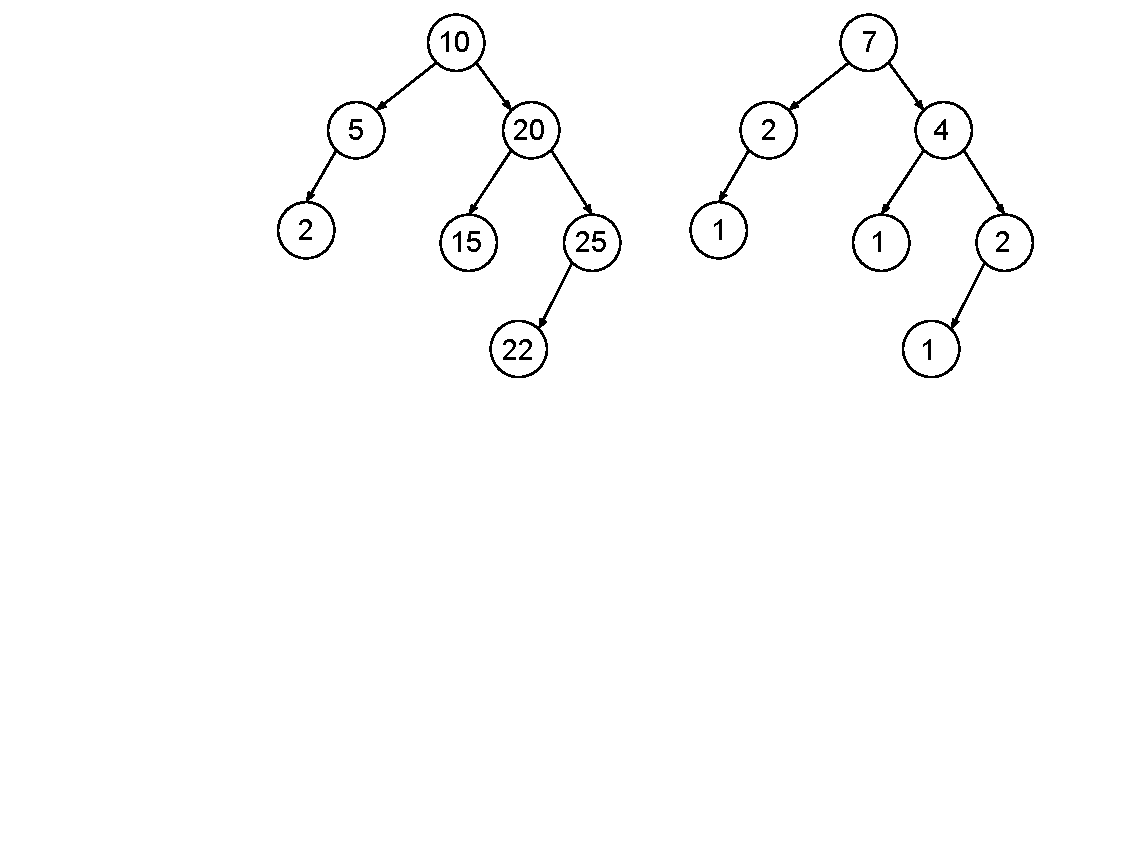
\includegraphics[width=4cm]{images/tree1}

	\caption{Двоично наредено дърво}
  \label{fig:tree1}
  \end{figure}


	\item Да се деифнира метод \texttt{countLeaves} на клас \texttt{BTree}, който намира броя на листата в дървото.

	\item Да се деифнира метод \texttt{maxLeaf} на клас \texttt{BTree}, който намира най-голямото по стойност листо на непразно дърво. Да се приеме, че за типа \texttt{T} на шаблона \texttt{BTree} е дефиниран операторът \texttt{<}.

	\item Нека е дадено дървото \texttt{t} и низът \texttt{s}, съставен само от символите `L' и `R' ($s \in \{L,R\}^*$). Нека дефинираме ``съответен елемент'' на низа \texttt{s} в дървото \texttt{t} по следния начин:
	\begin{itemize}
		\item Ако дървото \texttt{t} е празно, низът \texttt{s} няма съответен елемент
		\item Ако низът \texttt{s} е празен, а дървото \texttt{t} - не, то коренът на дървото \texttt{t} е съответният елемент на низа \texttt{s}
		\item Ако първият символ на низа \texttt{s} е `L' и дървото \texttt{t} не е празно, то съответният елемент на низа \texttt{s} в дървото \texttt{t} е съответният елемент на низа $s+1$ в \textbf{лявото} поддърво на \texttt{t}
		\item Ако първият символ на низа \texttt{s} е `R' и дървото \texttt{t} не е празно, то съответният елемент на низа \texttt{s} в дървото \texttt{t} е съответният елемент на низа $s+1$ в \textbf{дясното} поддърво на \texttt{t}
	\end{itemize}

	\textit{Пример. За 	дървото от Фигура \ref{fig:tree1}, съответният елемент на празния низ е 10, на низа ``RL'' е 15, а ``RLR'' няма съответен елемент.}

	Да се дефинира метод \texttt{T\& BTree<T>::getElement (const char *s)}, който намира съответния елемент на низа \texttt{s}. Какво връща методът в случаите на липса на съответен елемент е без значение.


\end{enumerate}

\subsection {Отпечатване и сериализация}

\begin{enumerate}[resume]

  \item Да се дефинира метод \texttt{void BTree<T>::prettyPrint ()}, отпечатващ дървото на конзолата по следния начин: (1) всеки наследник е вдясно от родителя си, (2) елементите на еднакво ниво в дървото се отпечатват на еднаква колона от екрана, (3) десните наследници са на предишен ред от родителя си и (4) левите наследни са следващ ред спрямо родителя си.

  Например, дървото от Фигура \ref{fig:tree1} би изглеждало по следния начин (включени са номерата на редовете на конзолата):

  \begin{verbatim}
  1:        25
  2:    20
  3:        15
  4: 10
  5:    5
  \end{verbatim}



  \item Да се дефинират методи за сериализация и де-сериализация на двоично дърво, като се използва ``\texttt{Scheme} формат''.
\end{enumerate}

\begin{mdframed}[hidealllines=true,backgroundcolor=gray!20]
Представяне на двоично дърво в ``Scheme формат'' наричаме еднозначно текстово представяне на структурата от данни, образувано по следните правила:
\begin{itemize}
  \item Празното дърво се прдставя с низа ``()''
  \item Нека е дадено дървото $t$ с корен $x$, ляво поддърво $t_l$ и дясно поддърво $t_r$. Ако $s_l$ е представянето в ``Scheme формат'' формат на $t_l$, а $s_r$ е представянето в ``Scheme формат'' на $t_r$, то низът ``($x$ $s_l$ $s_r$)'' е представянето на дървото $t$, кдето ``$x$'', ``$s_l$'' и ``$s_r$'' са съответните низове.

\end{itemize}
Например, дървото от Фигура \ref{fig:tree1} се представя по следния начин:

\begin{verbatim}
(10 (20 (25 () ()) (15 () ())) (5 () ()))
\end{verbatim}

\end{mdframed}

\subsection {Извличане на нескаларни свойства}
\begin{enumerate}[resume]

  \item Да се реализира метод \texttt{std::vector<T> BTree<T>::listLeaves ()} намиращ списък със стойностите на листата на дървото.

  \item Да се дефинира метод \texttt{std::string BTree<T>::findTrace (const T\& x)}. Ако \texttt{x} е елемент на дървото, функцията да връща следата на \texttt{x} (според дефиницията на ``следа'', обсъдена на лекции). Ако \texttt{x} не е елемент на дървото, функцията да връща низа ``\_''.

  \textit{Пример: За дървото от Фигура \ref{fig:tree1}, следата на елемента със стойност 25 е ``RR''}.

\end{enumerate}

\subsection{Итериране на елементите на двоично дърво}

\begin{enumerate}[resume]
  \item Да се дефинира оператор \texttt{T\& BTree<T>::operator[](int i)}, който намира $i$-тият пореден елемент на дървото при обхождане корен-ляво-дясно.

  Пример: За дървото от Фигура \ref{fig:tree1}, елементът с пореден номер 0 е 10, с номер 1 е 5, с номер 2 е 20 и т.н.
\end{enumerate}

\subsection {Представяне на аритметичен израз чрез дърво}
\begin{enumerate}[resume]
\item Нека е даден израз, построен по правилата на следната граматика:

\begin{verbatim}
<expression> ::= <digit> | (<expression><operator><expresson>)
<digit> ::= 1..9
<operator> ::= + | - | * | /
\end{verbatim}

Да се реалзира метод на клас \code{BTree<char>}, \code{void parseExpression (std::string s)}, който по правилно построен израз, записан в низа \texttt{s}, създава двоично дърво от символи, представящо израза по следното правило:
\begin{itemize}
  \item Ако изразът е от типа ``\texttt{x}'', където \texttt{x} е цифра, то съответното му дърво е листо със стойност символа \texttt{x}.
  \item Ако изразът е от типа ``\texttt{(<израз 1><op><израз 2>)}'', то съответното му дърво има като стойност на корена символа на съответния оператор, ляво поддърво, съответно на \texttt{<израз 1>} и дясно поддърво, съответно на \texttt{<израз 2>}.
\end{itemize}

Дървото на Фигура \ref{fig:treeexpr} съответства на изарза \code{(1*(2+3))}.

\begin{figure}
\centering
\begin{tikzpicture}[auto, node distance=2cm,>=latex']
\node [treenode] {*}
  child {
    node [treenode] {1}
  }
  child {
    node [treenode] {+}
    child {
      node [treenode] {2}
    }
    child {
      node [treenode] {3}
    }
  };
\end{tikzpicture}
\caption{Дърво на израза \code{(1*(2+3))}.}
\label{fig:treeexpr}
\end{figure}

\item Да се реализира метод \texttt{double BTree<char>::calculateExpresisonTree ()}, който намира стойността на израз, построен от решението на предишната задача.

\end{enumerate}

\subsection {Построяване и модификации на дърво}

\begin{enumerate}[resume]

  \item По дадено число $h$ да се построи идеално балансирано двоично дърво с височина $h$. Стойността на всеки от елементите на дървото да е равна на нивото, в което се намира елемента (вж. Фигура \ref{fig:balanced}).

  \begin{figure}
  \centering
  \begin{tikzpicture}[auto, sibling distance=5cm,>=latex',level 2/.style={sibling distance=3cm}]
  \node [] {0}
    child {
      node [] {1}
        child {
          node []{2}
        }
        child {
          node []{2}
        }
    }
    child {
      node [] {1}
      child {
        node []{2}
      }
      child {
        node []{2}
      }
    };
  \end{tikzpicture}
  \caption{Идеално балансирано двоично дърво с височина 3}
  \label{fig:balanced}
  \end{figure}

  \item {Нека е даден символен низ $s$ с дължина $n$. Нека $h$ е такова, че $2^h \geq n > 2^{h-1}$ } (минималната височина на двоично дърво, което има поне $n$ листа в последното си ниво). Да се дифинира функция, която по даден низ $s$ построява двоично дърво от символи с височина $h$, такова, че низът $s$ е разположен в листата на дървото, четени от ляво надясно. Възлите на дървото, които не са листа, да съдържат символа интервал. Вж. Фигура \ref{fig:stringleaves}

  \begin{figure}
  \centering
  \relscale{0.75}
  \begin{tikzpicture}[auto, sibling distance=8cm,>=latex',level 3/.style={sibling distance=5cm},level 2/.style={sibling distance=4cm},level 3/.style={sibling distance=2cm}]
  \node [treenode] {}
    child {
      node [treenode] {}
        child {
          node [treenode]{}
          child {
            node [treenode]{H}
          }
          child {
            node [treenode]{e}
          }
        }
        child {
          node [treenode]{}
          child {
            node [treenode]{l}
          }
          child {
            node[treenode] {l}
          }
        }
    }
    child {
      node [treenode] {}
      child {
        node [treenode]{}
        child {
          node [treenode]{o}
        }
        child {
          node [treenode]{!}
        }
      }
      child [missing]
    };
  \end{tikzpicture}
  \caption{Дърво, в чиито листа е разположен низът ``Hello!''}
  \label{fig:stringleaves}
  \end{figure}


  \item Стойността на всеки възел \texttt{V} в дадено двоично дърво от числа да се замени с броя на всички елементи на поддървото, на което \texttt{V} е корен. Вж. Фигура \ref{fig:treenodecount}. \emph{При операцията всеки от възлите да бъде посетен най-много веднъж!}

  \begin{figure}
  \centering
  \begin{tabular}{c c}
  \begin{tikzpicture}[auto, node distance=2cm,>=latex']
  \node [treenode] {10}
    child {
      node [treenode] {5}
      child {
        node [treenode] {2}
      }
      child [missing]
    }
    child {
      node [treenode] {20}
      child {
        node [treenode] {15}
      }
      child {
        node [treenode] {25}
        child {
          node [treenode] {22}
        }
        child [missing]
      }
    };
  \end{tikzpicture}
   &
   \begin{tikzpicture}[auto, node distance=2cm,>=latex']
   \node [treenode] {7}
     child {
       node [treenode] {2}
       child {
         node [treenode] {1}
       }
       child [missing]
     }
     child {
       node [treenode] {4}
       child {
         node [treenode] {1}
       }
       child {
         node [treenode] {2}
         child {
           node [treenode] {1}
         }
         child [missing]
       }
     };
   \end{tikzpicture}

  \end{tabular}
  \caption{Примерно дърво и същото дърво, стойностите на чиито възли са заместени с размера на съответното им поддърво}
  \label{fig:treenodecount}
  \end{figure}


  \begin{figure}
  \centering
  \relscale{0.7}
  \begin{tabular}{c c}

  \begin{tikzpicture}[auto, sibling distance=1.75cm,>=latex']
  \node [] {``this is a tree''}
    child {
      node [] {``which has''}
      child {
        node [] {``on its''}
        child {
          node [] {``your task''}
        }
        child [missing]
      }
      child {
        node [] {``nodes''}
        child {
          node [] {``is to have''}
        }
        child [missing]
      }
    }
    child {
      node [] {``strings''}
      child [missing]
      child {
        node [] {``and''}
        child {
          node [] {``fun with it''}
        }
        child [missing]
      }
    };
  \end{tikzpicture}
  &
  \begin{tikzpicture}[auto, sibling distance=5.5cm,>=latex',level 3/.style={sibling distance=1.5cm},level 2/.style={sibling distance=3cm}]
  \node [] {``this is a tree''}
    child {
      node [] {``which ha''}
      child {
        node [] {``on i''}
        child {
          node [] {``your''}
        }
        child {
          node [] {`` tas''}
        }
      }
      child {
        node [] {``ts n''}
        child {
          node [] {``k is''}
        }
        child {
          node [] {``to h''}
        }
      }
    }
    child {
      node [] {``sstrings''}
      child {
        node [] {``odes''}
        child {
          node [] {``ave ''}
        }
        child {
         node [] {``fun ''}
        }
      }
      child {
        node [] {``and''}
        child {
          node [] {``with''}
        }
        child {
          node [] {`` it''}
        }
      }
    };
  \end{tikzpicture}
  \end{tabular}
  \caption{Примерно дърво от низове преди и след балансирането}
  \label{fig:treeexpr}
  \end{figure}

  \item Дадено е дърво с низове по върховете. Дървото да се балансира по следния начин:

  \begin{enumerate}[label=\alph*)]
    \item Резултатното дърво има същия брой нива като изходното.
    \item Всяко $k$-то ниво на резултатното дърво да съдържа точно $2^k$ елемента (считаме, че коренът е на ниво 0).
    \item Нека $s_k$ е низът, получен при конкатенацията на всички низове на ниво $k$ на изходното дърво, обхождани от ляво надясно. Нека дължината на низа $s_k$ е $n_k$ символа. $i$-тият пореден елемент на нивото $k$ в резултатното дърво да съдържа $i$-тата поредна последнователност от $\lceil{n_k/{2^k}}\rceil$ на брой символи на $s_k$, освен най-десния, който съдържа последните ``останали'' символи от $s_k$. T.e. $s_k$ да се ``раздели'' поравно между елементите в резултатното дърво.
  \end{enumerate}

  На Фигура \ref{fig:treeexpr} са илюстрирани примерно изходно дърво и резултатът от балансирането му по горното правило. Всички елементи на ниво 1, освен последния, съдържат по $8=\lceil{16/2}\rceil$ символа. Всички елементи на ниво 2, освен последния, съдържат по $4=\lceil{14/4}\rceil$ символа и т.н.


  \emph{Упътване: предварително намерете вектора $(s_0,s_1,...,s_{h-1})$ и го използвайте за балансирането.}
  \begin{figure}
  \centering
	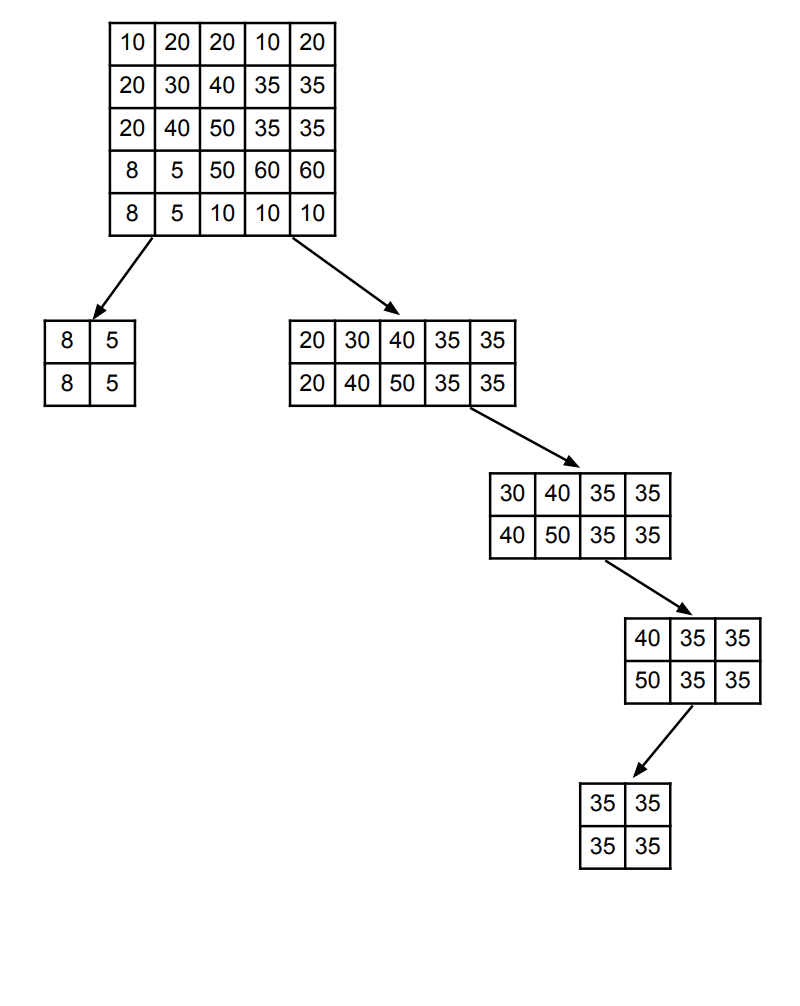
\includegraphics[width=9cm]{images/treematr}
  \caption{Наредено дърво от матрици}
  \label{fig:treematr}
  \end{figure}

  \item Нека е дадена матрица от цели числа $A_{M\times N}$ с елементи $(a_{i,j})$. ``Лява'' подматрица на $A$ наричаме такава подматрица $A'_{M'\times N'}$ на $A$, всеки елемент на която е по-малък от $a_{0,0}$. ``Дясна'' подматрица на $A$ наричаме такава подматрица $A'_{M'\times N'}$ на $A$, всеки елемент на която е по-голям от $a_{0,0}$.
  По дадена матрица $A$ да се построи двоично дърво $T$ със следните свойства:

	\begin{itemize}
		\item Коренът на $T$ съдържа матрицата $A$.
		\item Нека $v$ е произволен възел от дървото $T$, съдържащ матрица $X$. Ако $X$ има поне една лява подматрица с размер поне $2 \times 2$, то левият наследник на $X$ съдържа най-голямата (по брой елементи) лява подматрица на $X$. Ако има повече от една лявва подматрциа с максимален брой елементи, то левият наследник на $v$ е произволна една от тях. Ако $X$ няма лява подматрица с размер поне $2 \times 2$, то $v$ няма ляв наследник.
		\item Аналлогичното свойство за десния наследник на $v$ и най-голямата дясна подматрица (подматрици) на $X$.
	\end{itemize}

	На Фигура \ref{fig:treematr} е изобразено едно такова дърво.

	\begin{enumerate}[label=\alph*)]
		\item Да се избере подходящо представяне на матрици и на двоично дърво с матрици по върховете.
		\item Да се дефинира функция за построяване на дърво по горното правило по дадена матрица за корена му.
		\item Да се отпечата дървото чрез Graphviz. Повече информация за отпечатване на матрици като елемент на дървото може да се намери в \href{https://graphviz.gitlab.io/_pages/doc/info/shapes.html}{документацията на Graphviz}.
	\end{enumerate}


\end{enumerate}

\pagebreak

\section {Изображения (Maps)}
\subsection {HashMap}

\begin{mdframed}[hidealllines=true,backgroundcolor=gray!20]
Следнитте задачи са базирани на проста реализация на хеш таблица с отворено адресиране:
\begin{verbatim}
template <class KeyType, class ValueType>
class HashMap;
\end{verbatim}
Редовете в хеш таблицата са елементи от структурата:
\begin{verbatim}
template <class KeyType, class ValueType>
struct TableElement
{
  KeyType key;
  ValueType value;
  TableElement<KeyType,ValueType> *next;
}
\end{verbatim}
Самата хеш таблица е предтавена с член данната на класа \code{HashMap} \code{TableElement<KeyType, ValueType> **table}.
\end{mdframed}

\begin{enumerate}

  \item Да се дефинира метод \texttt{HashMap::efficiency()}, който изчислява ефективността на хеш таблицата като отношението  $\frac{all-coliding}{all}$, където $coliding$ е броят на ключовете, записани при колизия, а $all$ е броят на всички записани ключове.


  \item Да се дефинира оператор \texttt{<}\texttt{<} за клас \texttt{HashMap}, който отпечатва в поток всички двойки ключ-стойност в Хеш таблицата.

  \item Да се напише програма, която въвежда от клавиатурата две текста с произволна големина $t_1$ и $t_2$. Програмата да извежда броя на всички срещания на думи в $t_2$, които се срещат и в $t_1$.

  Пример: за следните текстове

  \textit{In computing, a hash table (hash map) is a data structure used to implement an associative array, a structure that can map keys to values. A hash table uses a hash function to compute an index into an array of buckets or slots, from which the correct value can be found.}

  и

  \textit{Ideally, the hash function will assign each key to a unique bucket, but this situation is rarely achievable in practice (usually some keys will hash to the same bucket)}

  Този брой е 10, съставен от думите \textit {the} (2 срещания във втория текст), \textit{a} (1 срещане), \textit{hash} (2), \textit {function} (1), \textit{to} (2), \textit{is} (1), \textit{keys} (1).


  \item Да се напише програма, която въвежда от клавиатурата две текста с произволна големина $t_1$ и $t_2$. Програмата да извежда броя на уникалните думи в $t_2$, които се срещат и в $t_1$.

  Пример: за двата текста от предишната задача, този брой е 7, съставен от думите \textit {the}, \textit{a}, \textit{hash}, \textit {function}, \textit{to}, \textit{is}, \textit{keys}.


  \item Да се напише програма, която прочита от входа даден текст с произволна големина и намира такава дума с дължина повече от 3 букви, която се среща най-често в текста. Пример: за текста

  \textit{In computing, a hash table (hash map) is a data structure used to implement an associative array, a structure that can map keys to values. A hash table uses a hash function to compute an index into an array of buckets or slots, from which the correct value can be found.}

  Най-често срещаната дума е \textit{hash}.

  \item От клавиатурата да се въведе цялото положително число $n$, следвано от $2 \times n$ цели положителни числа $a_1, b_1, a_2, b_2, ..., a_n, b_n$. Програмата да печата на екрана \texttt{``Yes''}, ако изображението, дефинирано като $h(a_i)=b_i,i=1,...,n$ е добре дефинирана функция. Т.е. програмата да проверява дали има два различни индекса $i$ и $j$, за които е изпълнено $a_i=a_j$, но $b_i \neq b_j$.

  \item Да се дефинира метод

  \texttt{void map ([подходящ тип] f)}

  на хеш-таблицата, който прилага функцията \texttt{f} над всички стойности в хеш-таблицата.

%begin с предикат

\end{enumerate}

\subsection{TrieMap}

\begin{figure}
\centering
\begin{forest}
for tree={align=center, inner sep=0pt, text centered, circle, font=\sffamily\bfseries, draw=black, fill=white, text width=1.5em }
[\_,
  [\_, edge label={node[midway,left] {\small{t}}}
    [7, edge label={node[midway,left] {\small{o}}}]
    [\_, edge label={node[midway,left] {\small{e}}}
      [3, edge label={node[midway,left] {\small{a}}}]
      [4, edge label={node[midway,left] {\small{d}}}]
      [12, edge label={node[midway,left] {\small{n}}}]
    ]
  ]
  [15, edge label={node[midway,right] {\small{A}}}]
  [11, edge label={node[midway,right] {\small{i}}}
    [5, edge label={node[midway,left] {\small{n}}}
      [9, edge label={node[midway,left] {\small{n}}}]
    ]
  ]
]
%edge label={node[midway,left] {\small{Help!}}}
\end{forest}
\caption{TrieMap, съдържащ двойките \code{to:7}, \code{tea:3}, \code{ted:4}, \code{ten:12}, \code{A:15}, \code{i:11}, \code{in:5} и \code{inn:9}.}
\label{fig:trie1}
\end{figure}


\begin{mdframed}[hidealllines=true,backgroundcolor=gray!20]
Следнитте задачи са базирани на проста реализация на речник (map) с ключове - символни низове и произволен тип на стойностите чрез префиксно дърво (Trie). Вж. Фигура \ref{fig:trie1}. Възлите в дървото съдържат указател към стойността на key-value двойката, а по дъгите на дървото са записани поредните букви от ключовете. Стойността е \code{nullptr} за междинните възли, които не съответстват на записан ключ. Наследниците на всеки възел са представени чрез \code{std::map<char,TrieNode*>} или някаква друга структура, която позволява наследникът да се ``анотира'' с буква:
\begin{verbatim}
template <class ValType>
struct TrieNode
{
  ValType *value;
  std::map<char,TrieNode<ValType>*> children;
};

template <class ValType>
class TrieMap
{
public:
  //...
private:
    TrieNode<ValType> *root;
};
\end{verbatim}
\end{mdframed}

\begin{enumerate}[resume]

	\item За клас \texttt{Trie} да се разработи приятелски клас \texttt{TrieUtilities}, който да реализира методи за:

	\begin{itemize}
		\item Намиране на височината на дървото.
		\item Намиране на дължината на най-дългия ключ, записан в дървото.
		\item Намиране на броя на записаните стойности в дървото.
		\item Намиране на броя на буквите на латинската азбука, които \emph{не учстват} в никой ключ на дървото.
	\end{itemize}

  \item Да се разработи оператор за индексиране (\texttt{[]}) на \texttt{Trie}, който да работи за четене и писане на ключове.

  \item Да се дефинира итератор за \texttt{Trie}, позволяващ обхождането на ключовете му в нарастващ ред относно лексикографската наредба.


	\item Да се реализира отпечатване на \texttt{Trie} в \texttt{dotty} формат.

\end{enumerate}

\pagebreak

\section {Декомпозиране на рекурсивни алгоритми с използване на стек}

\underline{Упътване}:Решете задачите с рекурсия и след това преобразувайте решението в решение със стек.


\begin{enumerate}

 \item (*)Да се дефинира функция за намиране на стойността на полинома на Ермит $Hn(x)$ (x е реална променлива, а n неотрицателна цяла променлива), дефиниран по следния начин:

 $H_0(x)=1$

 $H_1(x)=2x$

 $H_n(x)=2xH_{n-1}(x)+2(n-1)H_{n-2}(x), n>1$,

 за дадени $n$ и $x$ \underline{с използване на стек}.


 \item Нека е дадена абстрактна шахматна дъска с размери $n \times n$, $4 \le n \le 8$ и число $k$, $0 \le k \le n$. Казваме, че разположени на дъската  $k$ коня образуват ``валидна конфигурация'', ако никоя фигура не е поставена на поле, което се ``бие'' от друга фигура според съответните шахматни правила.

 Да се дефинира клас \texttt{KnightConfig}, представящ ``конфигуратор'' на шахматни коне. Конструкторът на класа инициализира конфигуратора с числата $n$ и $k$. Класът позволява ``обхождането'' една по една на всички валидни конфигурации за дадените параметри, по подобие на \texttt{forward} итератор на структура от данни. Класът да притежава следните методи:

 \begin{itemize}
   \item \texttt{void KnightConfig::printCurrentConfig()}: Отпечатва текущо намерената конфигурация.
     Пример за отпечатана конфигурация с $n=5, k=2$:
     \begin{verbatim}
     _ _ _ _ _
     _ _ H _ _
     _ _ _ _ _
     _ _ _ _ H
     _ _ _ _ _

     \end{verbatim}
   \item \texttt{void KnightConfig::findNextConfig()}: Намира следваща конфигурация.
   \item \texttt{bool KnightConfig::noMoreConfigs()}: Показва дали всички възможни конфигурации са вече изчерпани.
 \end{itemize}

 \item Да се реши задачата за Ханойските кули с използване на стек.

 Да се дефинира клас \texttt{HanoyPlayer} със следните методи:

 \begin{itemize}
   \item Конструктор с параметър, указващ броя дискове върху лявото колче за началното състояние на играта.
   \item Метод \texttt{bool final()}, който показва дали играта е достигнала финанлно състояние (т.е. всички дискове са на дясното колче).
   \item Метод \texttt{makeMove()}, който извършва един ход от играта.
   \item Метод \texttt{printBoard()}, който отпечатва текущото състояние на игровата дъска, например по следния начин:
     \begin{verbatim}

        2
        3     1
        5  *  4
     \end{verbatim}
   На примера е изобразено състояние на играта, при което на лявото колче има три диска - с размери 5, 3 и 2, на средното колче няма дискове, а на дясното има два диска - с размери 4 и 1.

 \end{itemize}



\end{enumerate}


\pagebreak

\begin{thebibliography}{99}

%\bibitem{sbornik}	Магдалина Тодорова, Петър Армянов, Дафина Петкова, Калин Георгиев, ``Сборник от задачи по програмиране на C++. Първа част. Увод в програмирането''

\end{thebibliography}

\end{document}
